% $Id: chapter3.tex 1790 2010-09-28 16:46:40Z jabriffa $

\chapter{System Analysis}

\section{Feasibility and System Limitations}
The project was designed as a demonstration to show how a let-alone, but personalized social news aggregator would work. The system flagship features of competing systems, all while mitigating issues such as the need of moderators to manage common issues such as vote-rigging or out-of-place content that disrupt the culture of the website.

Even though the system achieves the project's scope, that is not to say the system has reached its potential. There are many solutions that could perhaps increase the project's quality. For example, in order to improve sorting over time, the user could set their original interests but, over time a NN could monitor the user's actions and alter their interests judging from the way they interact with posts, such as time spent reading on a post that had other interests that the user did not initially mark as desirable. That way, the AI would create some hidden ranking that would sort the posts by that rank. It would not come with complications; nevertheless, building and running such a network would require not only immense dedicated computing power but also, periodic monitoring and safety regulation.

Changing the project's objectives and looking into lesser-known existing websites and their solutions in the literature review could likely provide more information on how these other systems handle sorting and what intricacies are involved when sorting information. Making the project more complex would defeat the goal of the project and could result in an overwhelming experience for the user. Moreover, in order for this project to yield meaningful results and an enjoyable experience results, responsiveness is key, which by overloading the system could result in the lack of those aspects.

\section{User Experience}
In order to create a user-friendly interface and experience, the front end of the website is going to use Boostrap. Bootstrap is a free and open-source CSS framework directed at responsive, mobile-first front-end web development. It contains CSS- and (optionally) JavaScript-based design templates for typography, forms, buttons, navigation, and other interface components \cite{wikipediacontributors_2019_bootstrap}. This allowed me to make a very clean and friendly user interface.

% \begin{figure}[!h]
%   \centering
% 	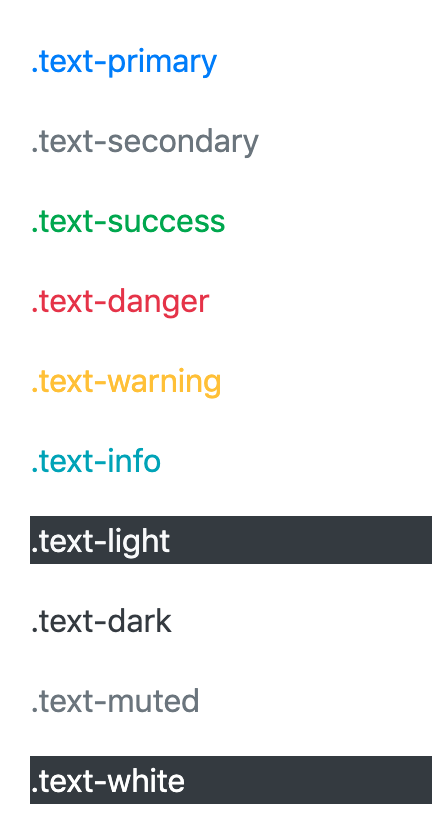
\includegraphics[scale=0.5]{Figures/bootstrap_colours}
% \caption{}
% \end{figure}

Bootstrap uses default colours for different types of importance as visible:

\begin{figure}[htbp]
\begin{minipage}[t]{0.45\linewidth}
    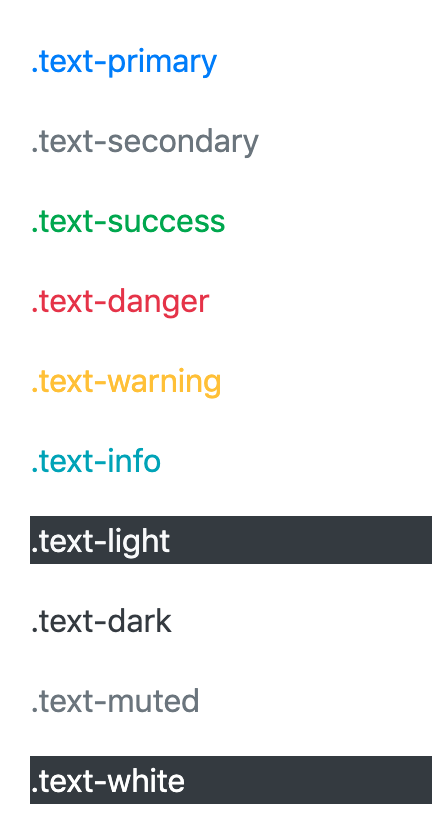
\includegraphics[scale=0.5]{Figures/bootstrap_colours}
    \caption{Bootstrap colours}
    \label{bootstrap_colours}
\end{minipage}%
    \hfill%
\begin{minipage}[t]{0.45\linewidth}
    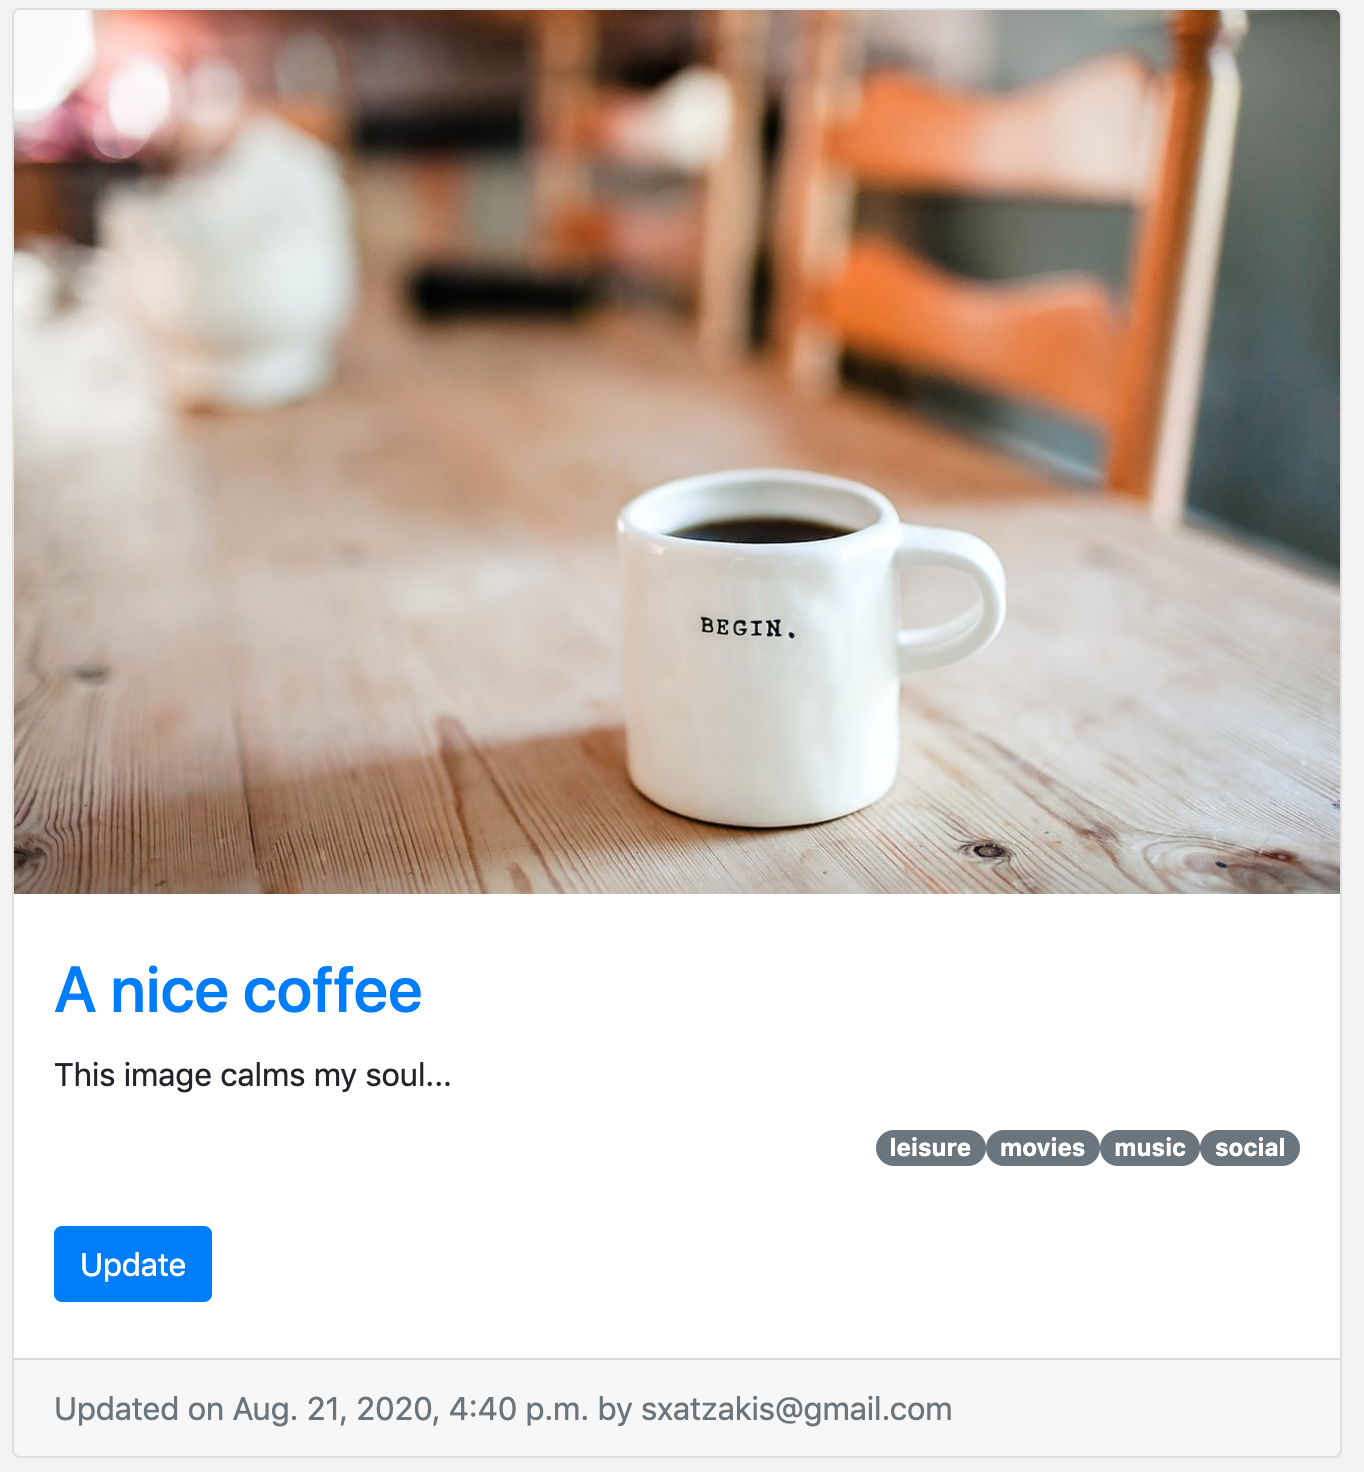
\includegraphics[width=\linewidth]{Figures/post_example}
    \caption{An example post}
    \label{example_post}
\end{minipage}
\end{figure}
% \begin{figure}[!htb]
%   \centering
% 	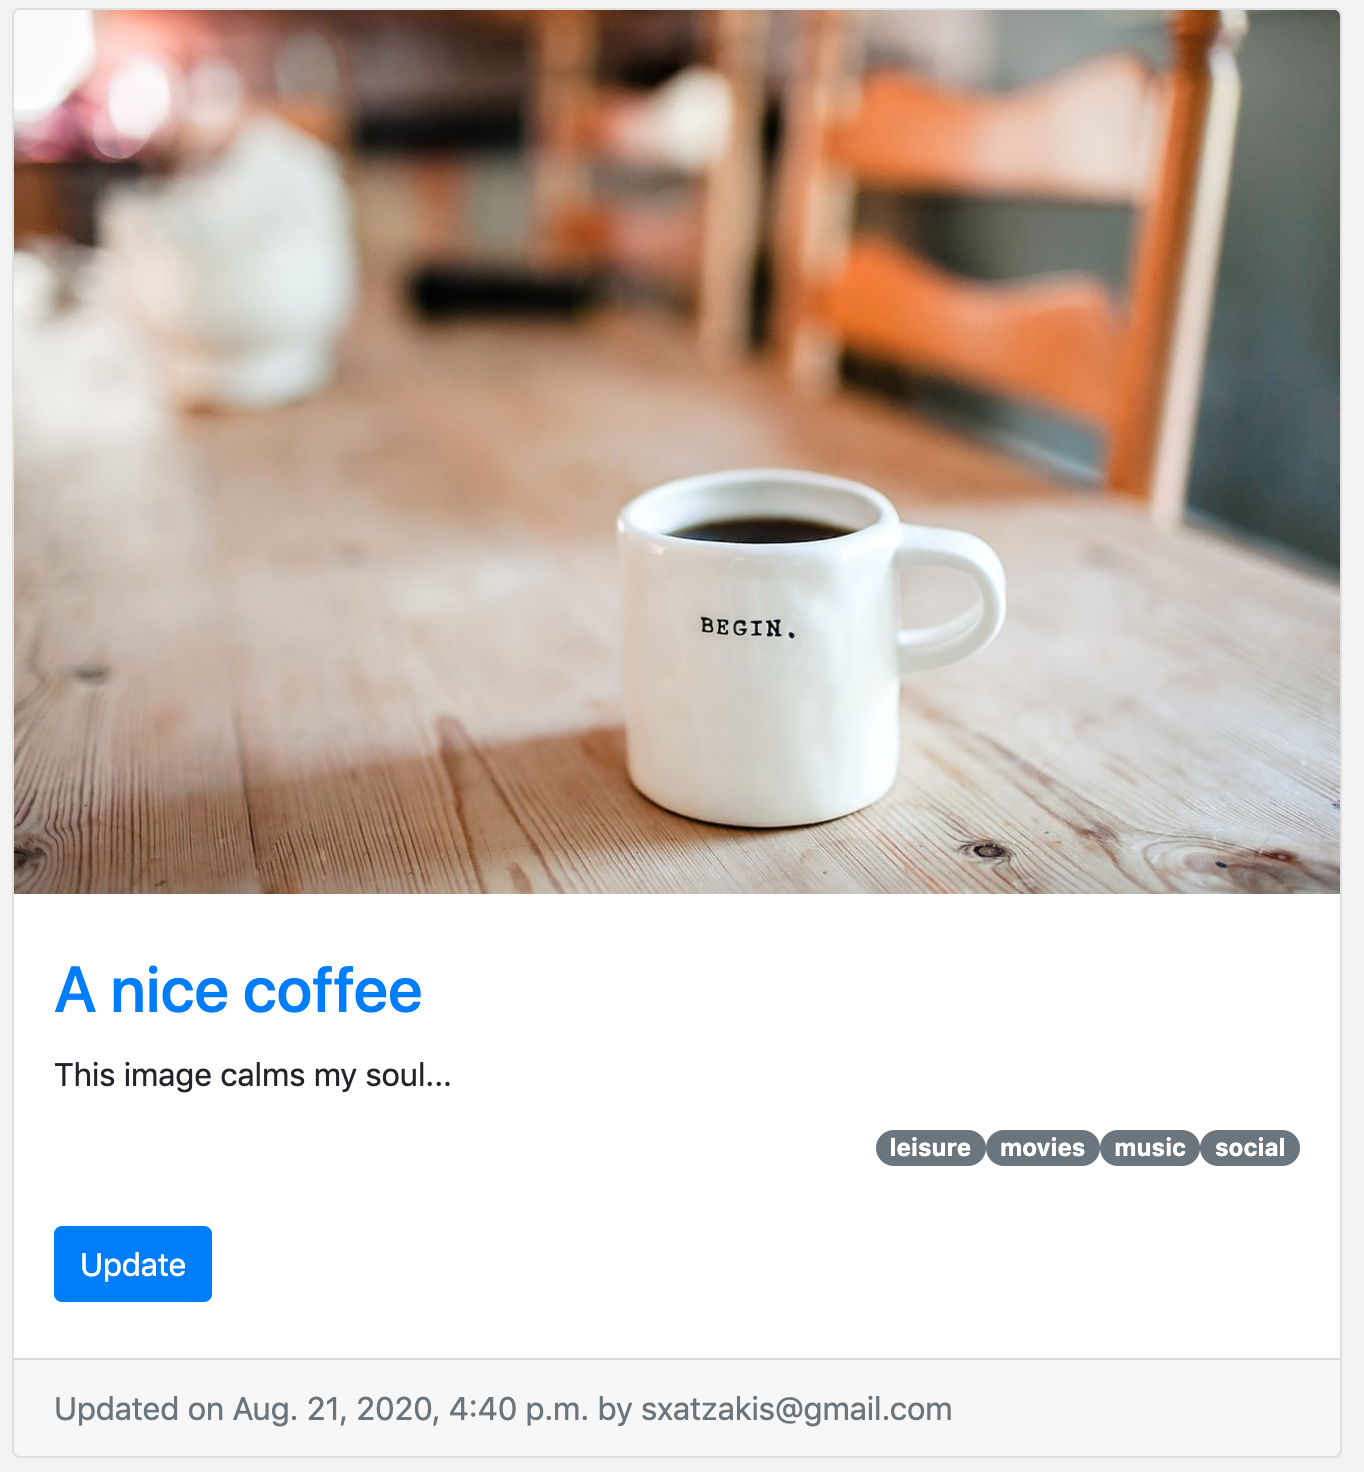
\includegraphics[scale=0.5]{Figures/post_example}
% \caption{}
% \end{figure}

\paragraph{}

After taking a few approaches, the final design I came up with was \ref{example_post}. Even though this is just a design, it should be easily linked to the back-end system. It consists of an image, a title, a body, an update button (if the post is by the user viewing it), several tags for the interests, and mutable text at the bottom with information on the post. The title is an important aspect of the post, meaning the blue colour was used to show importance. Next, the body text is plain text meaning it was left as is. The interest tags are not interactable meaning that the secondary colour of Bootstrap was used. The update button is a call to action; thus, used the primary colour. Lastly, the information below the post should be informative, and thus the muted colour was used. This style should be kept consistent throughout the website, giving the user a clear picture of what actions they can take at any point.

\section{System Requirements}

The project will be entirely written in Django; the back-end consists of Python and SQL, but the front-end is HTML meaning that the website should be available by any browser regardless of system specifications. Yet, in order to host the project, the host is required to meet a couple of specifications.

\subsection{Hosting Requirements}

Django includes requirements.txt files that includes the versions of the modules that it uses. In this case:

\begin{enumerate}
  \item Django==2.2.2
  \item Pillow==7.1.1
  \item pytz==2019.3
  \item sqlparse==0.3.1
\end{enumerate}

\paragraph{Specifications}

\begin{enumerate}
  \item A modern operating system (Windows 7 or 10, Mac OS X 10.11 or higher 64-bit, Linux: RHEL 6/7 64-bit)
  \item x86 64-bit CPU (Intel/AMD architecture)
  \item 4-GB RAM
  \item 5GB free disk space
\end{enumerate}

This list includes the requirements in order for the project to run smoothly. The most important requirement for a system to host this project is for Python to be runnable; once this requirement is met, the project will execute regardless of the specifications. Another issue to consider is that the Disk space requirement for this project will scale depending on the number of posts.

\subsection{System Functionality}
The user should be able to view the home page with all the blog posts sorted by time. The user can choose to register an account with an email, user name and password. If they are logged in, they have the option to view the homepage with a personalized view. Furthermore, the user has the option to view the account details, where they can edit their personal information, and interests, and view all the posts they have made. When creating a post, the user should be able to enter a title and body content, and chose an image and the posts, interests. Moreover, the user should view other user's posts but only be able to edit posts made by them. Lastly, the user should be able to log out at any point.
